\subsection{C$_{13}$ polyenal}

A second test was performed on the highly conjugated C$_{13}$ polyenal

\begin{center}
\begin{figure}[ht]
\begin{center}

\includegraphics[width=10cm]{02_localization/images/C13-molecule.eps}
\end{center}
\caption{\footnotesize The C$_{13}$ transoid polyenal molecule. }
\label{fig:C13-molecule}
\end{figure}
\end{center}

\vspace{-5mm}
Applications of the localization technique on polyenals have been performed
\cite{mp-101-1389-2003,cpl-372-22-2003,ijqc-97-688-2004}.
This class of molecules is of particular interest due to their role in
photobiology as chromophores \cite{jacs-118-7790-1996}.
Moreover, they are excellent model systems for studying
the interaction between the $\pi$ system of the carbonyl group and the
$\pi$ system of the unsaturated chain \cite{tetrahedron-34-3591-1978}. 

The cisoid-transoid energy difference for the aldehydic group has been
studied, by rotating by 180 degrees the C-C single bond. This evaluation
should be very weakly affected by the length of the polyene chain. The
distances (in $\mbox{{\AA}ngstrom}$) are r(C=O)=1.220, r(C-C)=1.450,
r(C=C)=1.350, r(C-H)=1.100.  All angles are 120 degrees.  The cut and freeze
denomination follows the analogy with shorter chain polyenals, as depicted
in Fig.~\ref{fig:C13-selection}.

\begin{center}
\begin{figure}[h!]
\begin{center}
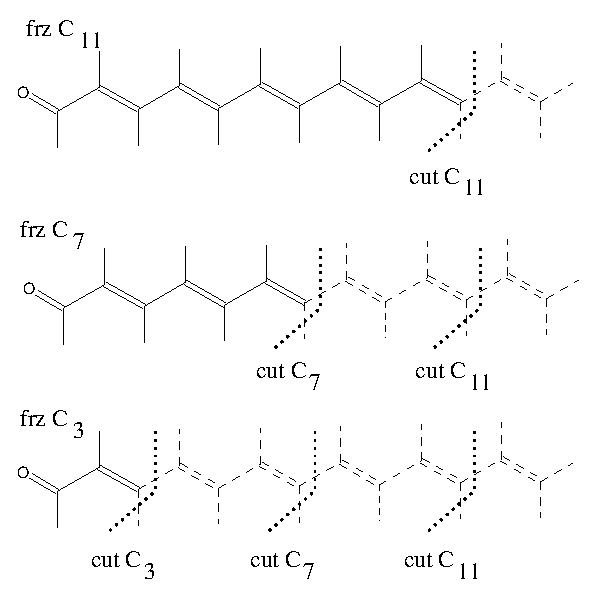
\includegraphics[width=8cm,keepaspectratio]{02_localization/images/C13-selection.eps}
\end{center}
\caption{\footnotesize C$_{13}$ polyenal molecule. Freeze and cut strategy
and labels follow the analogy with shorter chain polyenals. Localized
orbitals expressed on atoms of the dashed line framework are frozen.
Dotted lines depict the cut seam.  }
\label{fig:C13-selection}
\end{figure}
\end{center}


Two basis sets have been used: a minimal basis of type ANO-1 with $2s1p$
contraction for C and O, and a $1s$ contraction for hydrogen atoms
(hereafter named ANO-small), and a larger one ANO-1 with $3s2p$ contraction
for C and O, and a $2s$ contraction for hydrogens (ANO-large). As in the
previous case, the $1s$ core orbitals for carbon and oxygen atoms have been
frozen regardless of the freezing strategy.

Two CAS spaces have been considered. The first one, named CAS-A, contains
two electrons in the $\pi$/$\pi^{*}$ orbitals of the carbonyl group. The
second active space, named CAS-B, is defined as the previous one, further
extended with the inclusion of two additional electrons and the
$\pi$/$\pi^{*}$ orbitals from the double bond near the carbonyl. 

A preliminary evaluation with the ANO-small basis set and the CAS-A active
space has been performed on smaller polyenals, obtained by replacing the
removed part of the molecule with a hydrogen atom. The obtained results are
presented in Tab.~\ref{tbl:smaller-poly}.

\begin{center}
\begin{table}[ht]
\begin{center}
\footnotesize
\begin{tabular*}{0.75\textwidth}{l@{\hspace*{40mm}}ccc}
\hline
      	&    cisoid	&   transoid	  & diff	 \\
\hline
C$_{3}$ 	& -190.457653  	&	-190.460042   &	1.4981    \\
C$_{7}$ 	& -343.919126  	&	-343.921129   &	1.2563    \\
C$_{11}$	& -497.381057   &	-497.383042   &	1.2446    \\
C$_{13}$	& -574.112029   &	-574.114015   & 1.2453    \\
\hline
\end{tabular*}
\end{center}
\caption{\footnotesize CAS+S energy (Hartree) and difference (kcal/mol) between cisoid and
transoid complete structure for smaller polyenals, using the CAS-A active
space and the ANO-small basis set.}
\label{tbl:smaller-poly}
\end{table}
\end{center}


Tab. \ref{tbl:C13-cis-trans-diff} shows the absolute values for the CAS-A
with ANO-small basis set. Values are well reproduced, except when the cut is
near the frozen/non-frozen seam. This confirms the preceding statement
about this behavior. Also, the relative energies behave as expected. Again,
we can see that in the most pronounced Freeze-and-Cut strategy the results
are poor even in the relative energy.

Evaluation with the larger CAS-B (Tab.~\ref{tbl:C13-cis-trans-diff-casb})
and with the larger ANO-large basis set
(Tab.~\ref{tbl:C13-cis-trans-diff-ano-large}) show the same behavior.

Finally Fig. \ref{fig:C13-orbitals} shows the $\pi$ orbital for different cut
strategies, on the cisoid structure. Again, the Molden contour factor was
0.002, and the same behavior reported for the (7Z)-13 ammoniotridec-7-enoate
can be appreciated.  The cut-C11 strategy does not change the orbital in a
significant way, due to the graphically negligible expression of the
orthogonalization tail of the orbital on the removed part.  The other
strategies progressively restrict the orbital into the preserved part of
the polyenal.

\begin{center}
\begin{table}[ht]
\footnotesize
\begin{center}
\begin{tabular}{lcccc}
\hline                                                      
        &    nofrz       &    frz C$_{11}$      &   frz C$_{7}$        &   frz
C$_{3}$      \\
\hline                                                      
			&	\multicolumn{4}{c}{Cisoid} \\
nocut	&  -574.112029   &  -574.112025    &  -574.111981   & -574.110699   \\
cut C$_{11}$	&             	 &  -573.831612    &  -574.110383   & -574.110600   \\
cut C$_{7}$	&             	 &                 &  -573.826403   & -574.108770   \\
cut C$_{3}$	&             	 &             	  &                & -573.837474  	\\
			&	\multicolumn{4}{c}{Transoid} \\
nocut		&	-574.114015  	&	-574.114009  	&	-574.113945  	& -574.112686   \\
cut C$_{11}$&	             	&	-573.833584  	&	-574.112346  	& -574.112589   \\
cut C$_{7}$	&					&					&	-573.828399  	& -574.110797   \\
cut C$_{3}$	&					&					&					& -573.838137  	\\
			&	\multicolumn{4}{c}{Diff} \\
nocut			& 1.2453    &	1.2438    	&	1.2367    	&	1.2461    \\
cut C$_{11}$	&			&  	1.2367    	&	1.2314    	&	1.2474    \\
cut C$_{7}$		&			&				&  	1.2513    	&	1.2708    \\
cut C$_{3}$		&			&				&				&  	0.4161    \\
\hline
\end{tabular}
\end{center}
\caption{\footnotesize CAS+S absolute energies (Hartree) and energy
difference (kcal/mol) between cisoid and transoid C$_{13}$ polyenal using
the CAS-A active space and the ANO-small basis set, with respect to
different freeze and cut strategies.}
\label{tbl:C13-cis-trans-diff}
\end{table}
\end{center}

\begin{center}
\begin{table}[!ht]
\footnotesize
\begin{center}
\begin{tabular}{lcccc}
\hline
       &    nofrz       &    frz C$_{11}$      &   frz C$_{7}$        &   frz
C$_{3}$      \\
\hline                                                      
			&	\multicolumn{4}{c}{Cisoid} \\
nocut		&  -574.173041   &  -574.172995    	&  -574.172423   & -574.158115   \\
cut C$_{11}$&             	 &  -573.892623    	&  -574.170812   & -574.157975   \\
cut C$_{7}$	&             	 &                	&  -573.887517   & -574.156091   \\
cut C$_{3}$	&             	 &					&                & -573.889043  	\\
			&	\multicolumn{4}{c}{Transoid} \\
nocut		&	-574.174560  	&	-574.174521  	&	-574.174006  	& -574.160153   \\
cut C$_{11}$&	             	&	-573.894131  	&	-574.172393  	& -574.160015   \\
cut C$_{7}$	&					&					&	-573.889012  	& -574.158166   \\
cut C$_{3}$	&					&					&					& -573.888923  	\\
			&	\multicolumn{4}{c}{Diff} \\
nocut			& 0.9522    &	0.9567    	&	0.9919    	&	1.2776    \\
cut C$_{11}$	&			&  	0.9459    	&	0.9916    	&	1.2795    \\
cut C$_{7}$		&			&				&  	0.9378    	&	1.3015    \\
cut C$_{3}$		&			&				&				&  -0.0756    \\
\hline
\end{tabular}
\end{center}
\caption{\footnotesize CAS+S absolute energies and energy difference
(kcal/mol) between cisoid and transoid C$_{13}$ polyenal using the CAS-B
active space and the ANO-small basis set with respect to different freeze
and cut strategies.}
\label{tbl:C13-cis-trans-diff-casb}
\end{table}
\end{center}


\begin{center}
\begin{table}[!ht]
\footnotesize
\begin{center}
\begin{tabular}{lcccc}
\hline                                                      
        &    nofrz       &    frz C$_{11}$      &   frz C$_{7}$        &   frz C$_{3}$      \\
\hline                                                      
			&	\multicolumn{4}{c}{Cisoid} \\
nocut		&  -575.112195   &  -575.112194    	&  -575.112159   & -575.111082   \\
cut C$_{11}$&             	 &  -574.845588    	&  -575.108852   & -575.110774   \\
cut C$_{7}$	&             	 &                	&  -574.833700   & -575.106924   \\
cut C$_{3}$	&             	 &					&                & -574.850622  	\\
			&	\multicolumn{4}{c}{Transoid} \\
nocut		&	-575.115498  	&	-575.115500  	&	-575.115451  	& -575.114549   \\
cut C$_{11}$&	             	&	-574.848881  	&	-575.112168  	& -575.114263   \\
cut C$_{7}$	&					&					&	-574.837108  	& -575.110644   \\
cut C$_{3}$	&					&					&					& -574.849650  	\\
			&	\multicolumn{4}{c}{Diff} \\
nocut			& 2.0716    &	2.0738    	&	2.0644    	&	2.1742    \\
cut C$_{11}$	&			&  	2.0652     	&	2.0792    	&	2.1877    \\
cut C$_{7}$		&			&				&  	2.1369    	&	2.3328    \\
cut C$_{3}$		&			&				&				&  -0.6100    \\
\hline
\end{tabular}
\end{center}
\caption{\footnotesize CAS+S absolute energies and energy difference
(kcal/mol) between cisoid and transoid C$_{13}$ polyenal using the CAS-A
active space and the ANO-large basis set with respect to different freeze
and cut strategies.}
\label{tbl:C13-cis-trans-diff-ano-large}
\end{table}
\end{center}


\begin{figure}[!ht]
\begin{center}
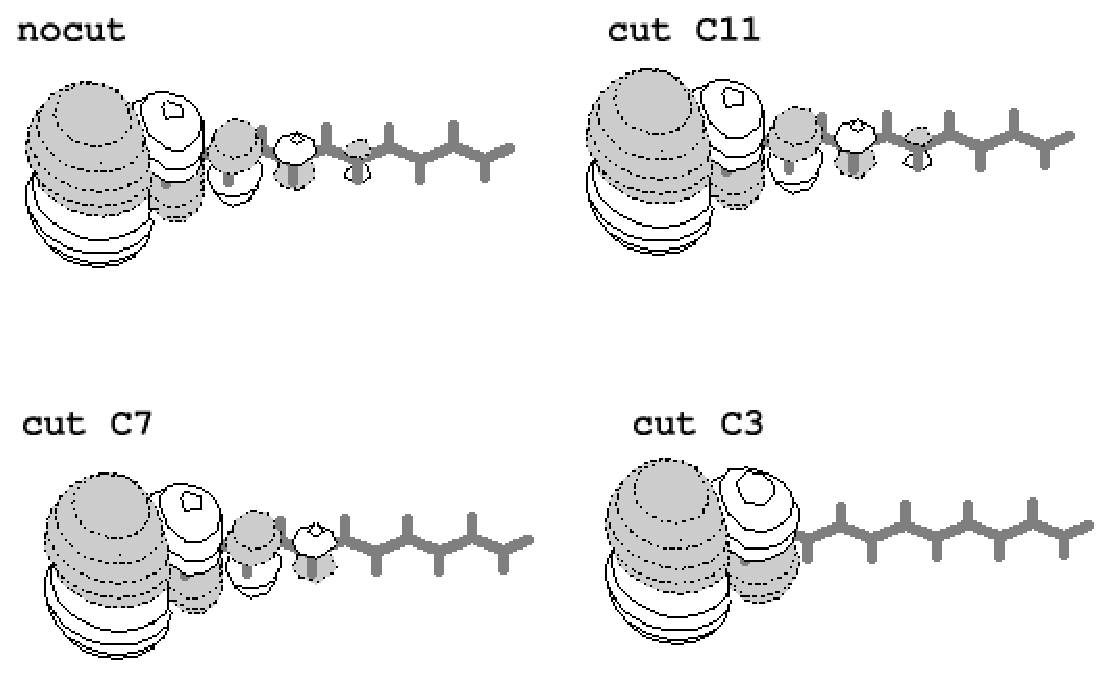
\includegraphics[width=8cm]{02_localization/images/C13-orbitals.eps}
\end{center}
\caption{\footnotesize The $\pi$ orbital for the C$_{13}$ cisoid polyenal with respect to
different cut strategies at frz-C$_{3}$ freeze strategy. The Molden contour factor for
the plot is 0.002. The progressive neglect of the orbital expression on
cut atoms can be appreciated.
}
\label{fig:C13-orbitals}
\end{figure}



\clearpage
